\documentclass[11pt]{article}
\usepackage[margin=0.8in]{geometry}
\usepackage{amsmath,amssymb,graphicx,tabularx,booktabs}
\usepackage[colorlinks=true,urlcolor=blue]{hyperref}
\setlength{\parindent}{0pt}\setlength{\parskip}{7pt}\setlength{\emergencystretch}{2em}
\begin{document}
{\LARGE Same-support validity: checked components}\par
{\large Mathematical component report, 2026-10-30}\par
\textbf{Coefficient result.} Lean accepted the polynomial coefficient implication below, and a separate readback reported its full type and axioms. Independent source review found the statement faithful to the bounded algebraic claim. The theorem is
\texttt{SameSupportCandidate.validity\_coefficients}.

Over a field $K$, let $u=X^2+qX+r$ and $v_i=s_iX+t_i$. For arbitrary $f\in K[X]$, assume
\[
 u\mid f-v_1^2,\qquad u\mid f-v_2^2,\qquad s_1=s_2.
\]
Then
\[
(t_2-t_1)(s_1+s_2)=0,\qquad (t_2-t_1)(t_2+t_1)=0.
\]
The divisibilities use the same $f$ and the same monic quadratic $u$. Odd characteristic, smoothness and a prescribed degree of $f$ are not hypotheses of this coefficient theorem.

\textbf{Proof structure.} Subtracting the two divisibilities shows that $u$ divides $v_2^2-v_1^2$. Equal slopes cancel the quadratic term, leaving
\[
D=(t_2-t_1)(s_1+s_2)X+(t_2-t_1)(t_2+t_1).
\]
Since $\deg u=2$ and $\deg D\le1$, divisibility forces $D=0$. Extracting coefficients one and zero gives the conjunction. The accepted correction changes an elaborator argument name and supplies explicit elementary coefficient identities; it adds no mathematical hypothesis.

\textbf{Abstract classifier composition.} The separate declaration
{\small\texttt{valid\_inputs\_exclude\_same\_support\_error}} composes this result with the existing abstract classifier. It assumes $\operatorname{Field} K$, decidable equality, $2\ne0$ and both common-support divisibilities. Equal slopes are not an extra premise: the proof splits on slope equality. The equal case applies the coefficient theorem and classifier helper; the unequal case follows the classifier's branch order. Its conclusion excludes the constructor \texttt{sameUMixedZeroSlope}.

\textbf{Classifier checks.} Candidate 4 compiled with exit 0, followed by a separate successful type-and-axiom readback. Its compile receipt binds the imported coefficient and helper objects by SHA-256. Independent source review reports \emph{holds / faithful scoped}; that reviewer did not read producer compiler output. This establishes two separately evidenced components: the normalized polynomial implication and its abstract classifier composition.

\textbf{Independent machine replay.} A second private directory rebuilt both helpers, the coefficient theorem and classifier corollary, then ran a separate declaration/axiom readback. All five native exits were zero. Its search path used fresh local objects plus the hashed dependency mirror, excluding the producer's helper directory. It reused the pinned Lean 4.34.1 toolchain and dependency binaries; no separate kernel rechecker was used.


\textbf{Axiom readback.} Accepted declarations report only \texttt{propext}, \texttt{Classical.choice}, and \texttt{Quot.sound}. Failed elaborations remain separately recorded; their intermediate output is not used as accepted theorem evidence.

\newpage
{\Large Checks, assumptions and the next concrete bridge}

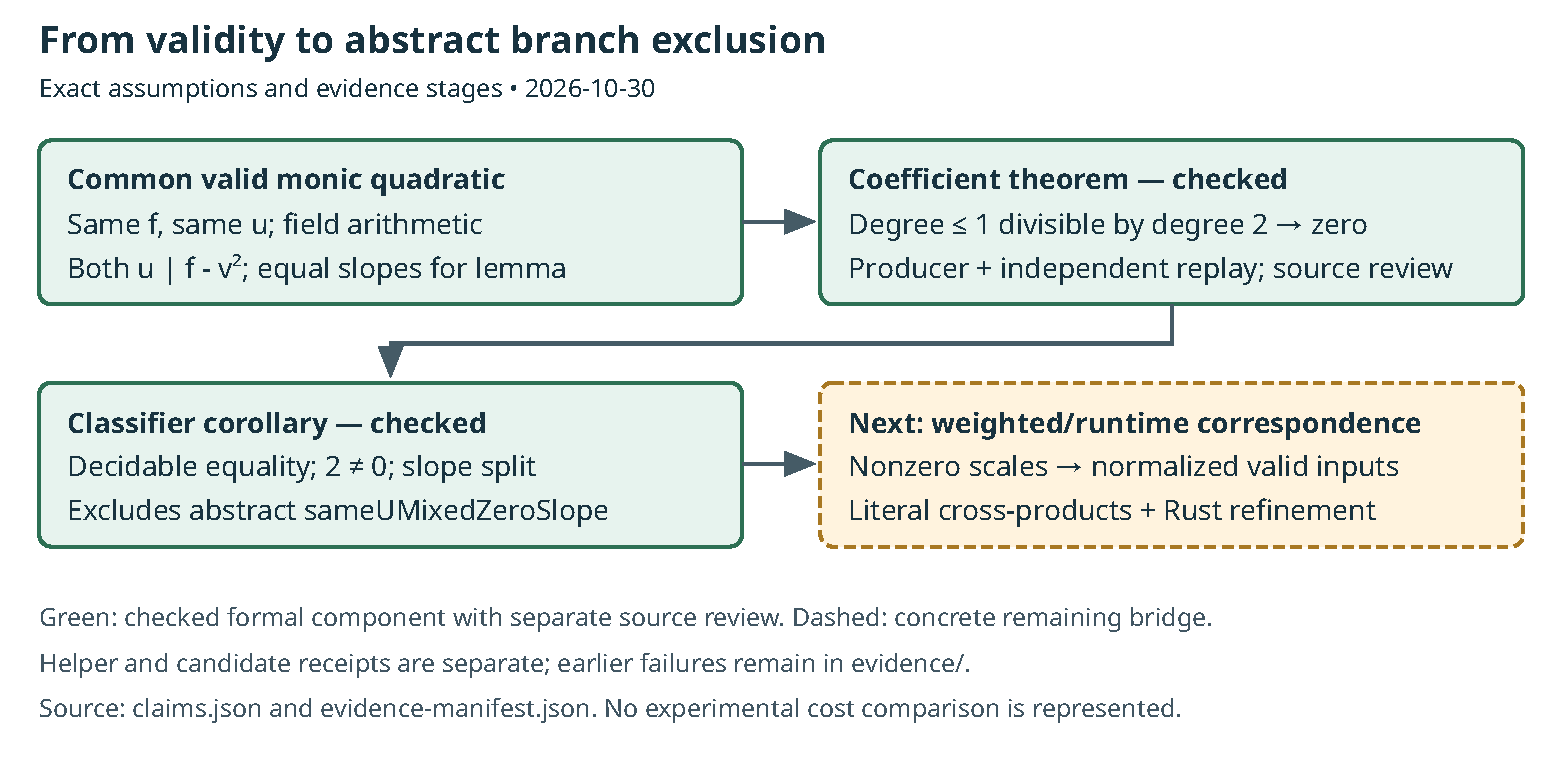
\includegraphics[width=\textwidth]{dependencies.pdf}

\textbf{Separated checks.} The helper modules, coefficient candidate and classifier candidate have separate compiler/readback receipts. Independent fidelity review reads statements and proof source without producer compiler output. The report combines those two evidence streams without relabelling the source-only review as a kernel run. Exact files, hashes and outcomes are in \texttt{claims.json} and \texttt{evidence-manifest.json}.

\textbf{Next bridge.} For literal weighted coordinates, prove in Lean that nonzero $z_i,w_i$ normalize to the valid common-support inputs and that the source cross-products satisfy, with $Z=z_1z_2$ and $W=w_1w_2$,
\[
Q_{ci}=Z^2\bar q_i,\quad R_{ci}=Z^4\bar r_i,\quad
S_{ci}=Z^3W\bar s_i,\quad T_{ci}=Z^5W\bar t_i.
\]
These identities turn the coefficient products into their runtime-scaled forms using $Z^8W^2$ and $Z^{10}W^2$. The written derivation already states this connection. It remains distinct from the checked normalized classifier theorem and from refinement to the compiled Rust arithmetic and exceptional branches. Establishing the required input invariant and preserving it through calls is part of that source-refinement work.

\textbf{Domain.} The checked classifier is an abstract field classifier; it is not an assertion that arbitrary tuples satisfy the Mumford validity premises. A global divisor-class addition theorem has further obligations beyond this branch exclusion.

\newpage
{\Large Operational record and reproducible review inputs}

\begin{tabularx}{\textwidth}{@{}p{0.31\textwidth}X@{}}\toprule
Recorded operation & Outcome retained\\\midrule
Original remote-cache helper & 120-second cap; RPC-backed cache wait; candidate not reached. Owned processes subsequently reaped.\\
Local mirror & 15,160 files, 2,274,679,663 bytes; recorded copy duration 274.474325 seconds; readback verified.\\
First local helper attempt & Exit 1, 3.001380 seconds; missing \texttt{Init.MethodSpecsSimp.olean}.\\
Second local replay & Boundary helper exit 0 (20.004973 seconds); runtime helper exit 0 (1.844236 seconds). Original candidate exit 1 (5.690498 seconds), elaboration errors.\\
Additional dependency copy & 1,392 files, 216,209,602 bytes; recorded duration 14.509870 seconds; readback verified.\\
Candidate attempt 3 & Exit 1 (3.489243 seconds); original source retained.\\
Coefficient attempt 3b & Corrected source compiled, exit 0 (1.500097 seconds), with separate successful type/axiom readback.\\\bottomrule
\end{tabularx}

These durations and copy sizes are operational records from their individual receipts. They are not a controlled timing comparison and are not summed into a performance claim. Prior failed output that mentions \texttt{sorryAx} is retained as failure evidence, separately from the accepted candidate's axiom readback.

\textbf{Packet contents.} \texttt{claims.json} contains named claims, exact assumptions, check outcomes and the remaining bridge. \texttt{evidence-manifest.json} binds copied source, readback, review and failure records. The \texttt{evidence/} tree preserves those small review inputs without copying the dependency cache. \texttt{dependencies.svg} and this LaTeX source are editable. Original immutable receipts remain unchanged; this report is an additive communication artifact.

\textbf{Review scope.} No research trial, scientific benchmark, cloud job or official evidence promotion was performed in generating this report. The sources and compiler outcomes belong to the named bounded formal components. Report generation itself performs no Lean compilation or experimental calculation.
\end{document}
